% !TeX root = ../MADRE-AgenticSystem.tex

\madreChapter{Conceptual Architecture}

\section{Formal Requirements}

This chapter states architectural requirements at product level.\n

\begin{tabularx}{.95\linewidth}{@{}lX@{}}
	\toprule
	\textbf{Requirement} & \textbf{Architectural meaning} \\
	\midrule
	\textbf{Local-first operation }& The kernel must be able to run useful workflows on local user-owned infrastructure before optional remote integrations are considered. \n
	\textbf{Model agnosticism }& All model execution enters through \texttt{ModelAction}, allowed \texttt{ModelBinding}, replaceable model-use profile, and model backend contracts, never through a vendor-specific core design. \n
	\textbf{Delayed reasoning }& The runtime must separate immediate conversation from deeper work that needs decomposition, evidence, verification, internal actions, or more compute. \n
	\textbf{Context governance} & Context must be selected, minimized, classified, provenanced, scoped, and revocable before it reaches models or internal actions. \n
	\textbf{Bounded internal actions }& Executable behavior must be declared, policy-checked, traceable, and constrained by side effect and recovery rules. Typed runtime-defined internal actions are the canonical low-risk action form. \n
	\textbf{\parbox{10em}{Record/knowledge isolation} }& retained interaction material, \texttt{KnowledgeRecord}, untrusted source material, \texttt{KnowledgeCandidate}, and \texttt{LearningCandidate} must not collapse into one undifferentiated prompt store. \n
	\textbf{Learning control }& A \texttt{LearningCandidate} is an evaluated proposed improvement and changes active module behavior only through a defined promotion boundary; storing a \texttt{KnowledgeRecord} is not learning. \n
	\textbf{Inspectable execution }& The CLI, local developer console, \texttt{RuntimeJournal}, and read models must make runtime behavior understandable without bypassing policy. \\
	\bottomrule
\end{tabularx}

\section{High-Level Architecture}

\Madre is organized around a deterministic runtime kernel that coordinates governed reasoning modules through responsibility boundaries rather than through a fixed topology.

The central architectural rule is simple: the model is never the system. Models are invoked through \texttt{ModelAction} under context, policy, action, knowledge, and trace constraints. Each concrete \texttt{MADREAgent} is owned by one \texttt{ReasoningModule} and constrained by \texttt{ModelBinding}. Agents may be short-lived, persistent, specialized, conservative, speculative, or workflow-bound, but they do not own the kernel or carry module knowledge across ownership boundaries.

The kernel coordinates modules; it does not become the reasoning actor for every task. System-level reasoning belongs in governed modules. Kernel registration assigns one compatible \texttt{ReasoningModule} the Core Module role for incoming interaction, continuity, clarification, planning, delegation, and delayed-work decisions. Within that module, one module-owned \texttt{SystemAgent} holds the Main Agent role; other \texttt{ComplexAgent} objects may exist without holding that role.

\subsection{Conceptual Components}

\begin{tabularx}{.95\linewidth}{@{}lX@{}}
	\toprule
	\textbf{Component} & \textbf{Responsibility} \\
	\midrule
	Access surfaces & Present the system through CLI, local read-first inspection console, graphical UI, speech, or domain applications without becoming the source of runtime authority. \n
	Core Module & A kernel-assigned \texttt{ReasoningModule} role that maintains interaction continuity, clarifies intent, creates reasoning plans, delegates to modules, and decides when deeper work is needed. \n
	Runtime kernel & Coordinates module registration, routing, scheduling, resource limits, policies, action registries, durable records, recovery, and lifecycle. \n
	Reasoning modules & Execute bounded reasoning domains through module-owned agents, workflows, routines, actions, records, policies, known-material boundaries, and allowed model/inference scope. \n
	Context and knowledge & Provides scoped context bundles and \texttt{KnowledgeRecord} objects with provenance, scope, sensitivity, intended use, truth metadata, and correction paths. \n
	Local Model Runtime Boundary & Product-level boundary for local or explicitly authorized inference through \texttt{ModelBinding}, model-use profile, model backend, \texttt{RuntimeEvent} evidence, and generated material. \n
	Agent Action boundary & Exposes typed, bounded internal actions with declared inputs, outputs, side-effect class, policy requirements, trace evidence, and recovery expectations. External actions are exceptional risk boundaries, not the default execution path. \n
	Learning and evolution & Evaluates \texttt{LearningCandidate} objects and promotes only authorized module improvements; known-material storage is separate. \n
	Observability and recovery & Gives developers and authorized users a read-first view of \texttt{ReasoningTask}, \texttt{RuntimeEvent}, \texttt{PolicyDecision}, failures, and rollback options through \texttt{RuntimeJournal}. \\
	\bottomrule
\end{tabularx}
\subsection{Responsibility Layer Diagram}

Figure~\ref{fig:madre-responsibility-layers} presents the primary responsibility structure of \Madre. The diagram is not a sequential request pipeline. It describes the ownership boundaries that constrain all runtime behavior.

The \Madre runtime kernel is the deterministic system coordinator. It owns access-surface entry, module registration, Core Module assignment, module routing, scheduling, resource assignment, global policy boundaries, \texttt{RuntimeJournal} coordination, durable runtime state, and lifecycle boundaries. The kernel does not become the reasoning actor for ordinary tasks. It selects, activates, limits, and observes reasoning modules.

Reasoning modules are the runtime units that perform domain-bounded reasoning. The module assigned the Core Module role is the first receiver for ordinary user interaction because its registered capability covers interaction continuity, clarification, general planning, and delegation. Other modules may specialize in research, knowledge handling, code, media, resource optimization, or domain-specific work. A module may answer quickly, create delayed work, invoke internal actions, or evaluate outcomes when its local policy and assigned resources allow it.

Executable behavior is not exposed as arbitrary external tools. The normal execution path uses an Agent Action boundary composed of typed runtime-defined functions with declared inputs, outputs, side-effect class, policy requirements, \texttt{RuntimeEvent} trace obligations, and recovery expectations. The first reference implementation may implement these actions on a JVM runtime, but JVM binding is not an architecture-level authority. External services, host commands, provider-backed tools, remote model services, or arbitrary plugin surfaces are not part of the default path and require stronger authority boundaries.

The Local Model Runtime Boundary is useful product-level phrasing for the point below the module and action layer where allowed inference executes. It is realized through \texttt{ModelBinding}, model-use profile, model backend, \texttt{RuntimeEvent} evidence, and generated material; it is not a chatbot server or an authority. Generated material returns to the module as generated material and is not truth, policy, memory, knowledge, behavior, routing, authority, or a candidate by itself.


\subsection{Concurrent Agent Lanes}

\Madre separates immediate interaction from deeper reasoning, but this separation is not modeled as two global subsystems. It is a possible execution pattern for a module-owned \texttt{MADREAgent}.

A \texttt{MADREAgent} with a \texttt{ComplexAgent} profile may maintain three concurrent lanes. The foreground lane preserves conversational continuity, answers only when safe known context is sufficient, asks for clarification when intent or risk is unclear, and creates deferred work when more evidence is required. The reasoning lane performs planning, decomposition, evidence gathering, action invocation, verification, and result construction under module authority. The reflection lane reviews recent work, observes delayed outcomes, detects failure patterns, and proposes evaluated \texttt{LearningCandidate} objects.

This pattern may exist in any reasoning module. The Core Module may use it for general interaction and delegation. A research module may use it for evidence comparison and verification. A knowledge module may use it for extraction, provenance checks, correction, and deletion semantics. The kernel schedules and constrains these lanes through module routing, resource limits, durable state, policy, and \texttt{RuntimeJournal}, but the reasoning behavior itself belongs to module-local agents.

\section{Runtime Data Flow}

Runtime data flow in \Madre is concurrent, governed, and module-centered. A local request enters through an access surface and is submitted to the kernel. The kernel records the request, applies the relevant entry policy, and routes it to the Core Module by registration or to another registered module when routing evidence supports that decision.

Within the selected module, its Main Agent role may produce an immediate foreground response, create or continue delayed reasoning work, invoke internal actions, request inference through an allowed \texttt{ModelAction}, and reflect on recent outcomes. These activities are coordinated inside a module-owned agent and constrained by module policy, kernel policy, \texttt{ModelBinding}, resource assignment, durable state, \texttt{RuntimeJournal}, and recovery rules.

The following subsections describe the canonical request narrative, the governed model/action sequence, and the data-authority rules that prevent user input, source material, generated material, action results, or learning candidates from promoting themselves into authority-bearing state.

\subsection{Canonical Request Narrative}

The canonical user request begins when an access surface submits a local request to the kernel. The kernel does not interpret the request as a \texttt{KnowledgeRecord}, factual authority, or policy. It records a \texttt{RuntimeEvent}, applies entry constraints, and routes the work to the Core Module unless another module is already selected by session state, policy, or module registry evidence.

The receiving module evaluates the request through its module-local Main Agent role. If a configured foreground lane has enough safe local context, it may produce an immediate answer. If intent, scope, or risk is unclear, it asks for clarification. If the request requires evidence, stronger reasoning, internal actions, model inference, or broader context, the reasoning lane creates or continues a \texttt{ReasoningTask}. Reflection may run after the response or after delayed outcomes to propose a \texttt{LearningCandidate}. Knowledge-boundary change is separately represented as a \texttt{KnowledgeCandidate}.

Every significant step emits a \texttt{RuntimeEvent} through \texttt{RuntimeJournal}. Context bundles, actions, \texttt{RuntimeEvent} evidence and generated material objects, \texttt{PolicyDecision} outcomes, failures,
corr ection, rollback, invalidation, supersession, and deletion/detachment remain inspectable through read-first surfaces.

\subsection{Governed Model And Action Sequence}

When module work requires executable behavior, the module invokes an internal typed action. The default action mechanism is local, typed, runtime-defined, policy-gated, and traceable. It is not an open plugin socket and not a network-exposed external action protocol.

A \texttt{ModelAction} is an \texttt{AgentAction} that uses inference. Before it runs, the module supplies a governed \texttt{ContextBundle}, an allowed \texttt{ModelBinding} and model-use profile, and the applicable \texttt{PolicyDecision}. An model backend executes inference without allowing a provider, template, or runtime format to define \Madre's authority model. One execution is captured as an \texttt{RuntimeEvent} evidence; its generated material is an generated material.

Action results may be observations. generated material is generated material and is not a candidate by itself. It may inform a next reasoning step or undergo explicit handling into another record, but it does not authorize actions, create policy, become memory or knowledge, change routing or behavior, or promote learning. Each such transition requires its relevant authority boundary, verification path, \texttt{RuntimeEvent} record, and recovery expectation.

% Shared TikZ requirements
 \usetikzlibrary{positioning,fit,backgrounds,arrows.meta,calc}

\tikzset{
	madrebox/.style={
		draw,
		rounded corners=2pt,
		align=center,
		minimum height=0.85cm,
		inner sep=5pt,
		font=\small
	},
	madreKernel/.style={madrebox, thick, fill=gray!10},
	madreModule/.style={madrebox, thick, fill=blue!6},
	madreAgent/.style={madrebox, thick, fill=orange!8},
	madreData/.style={madrebox, fill=purple!6},
	madreAction/.style={madrebox, fill=green!7},
	madrePolicy/.style={madrebox, fill=red!6},
	madreBoundary/.style={
		draw,
		dashed,
		rounded corners=4pt,
		inner sep=8pt
	},
	madreFlow/.style={->, thick, >=Latex},
	madreAsync/.style={->, thick, dashed, >=Latex},
	madreObserve/.style={->, dotted, thick, >=Latex}
}
\begin{figure}[H]
	\centering
	\resizebox{1.05\linewidth}{!}{%
		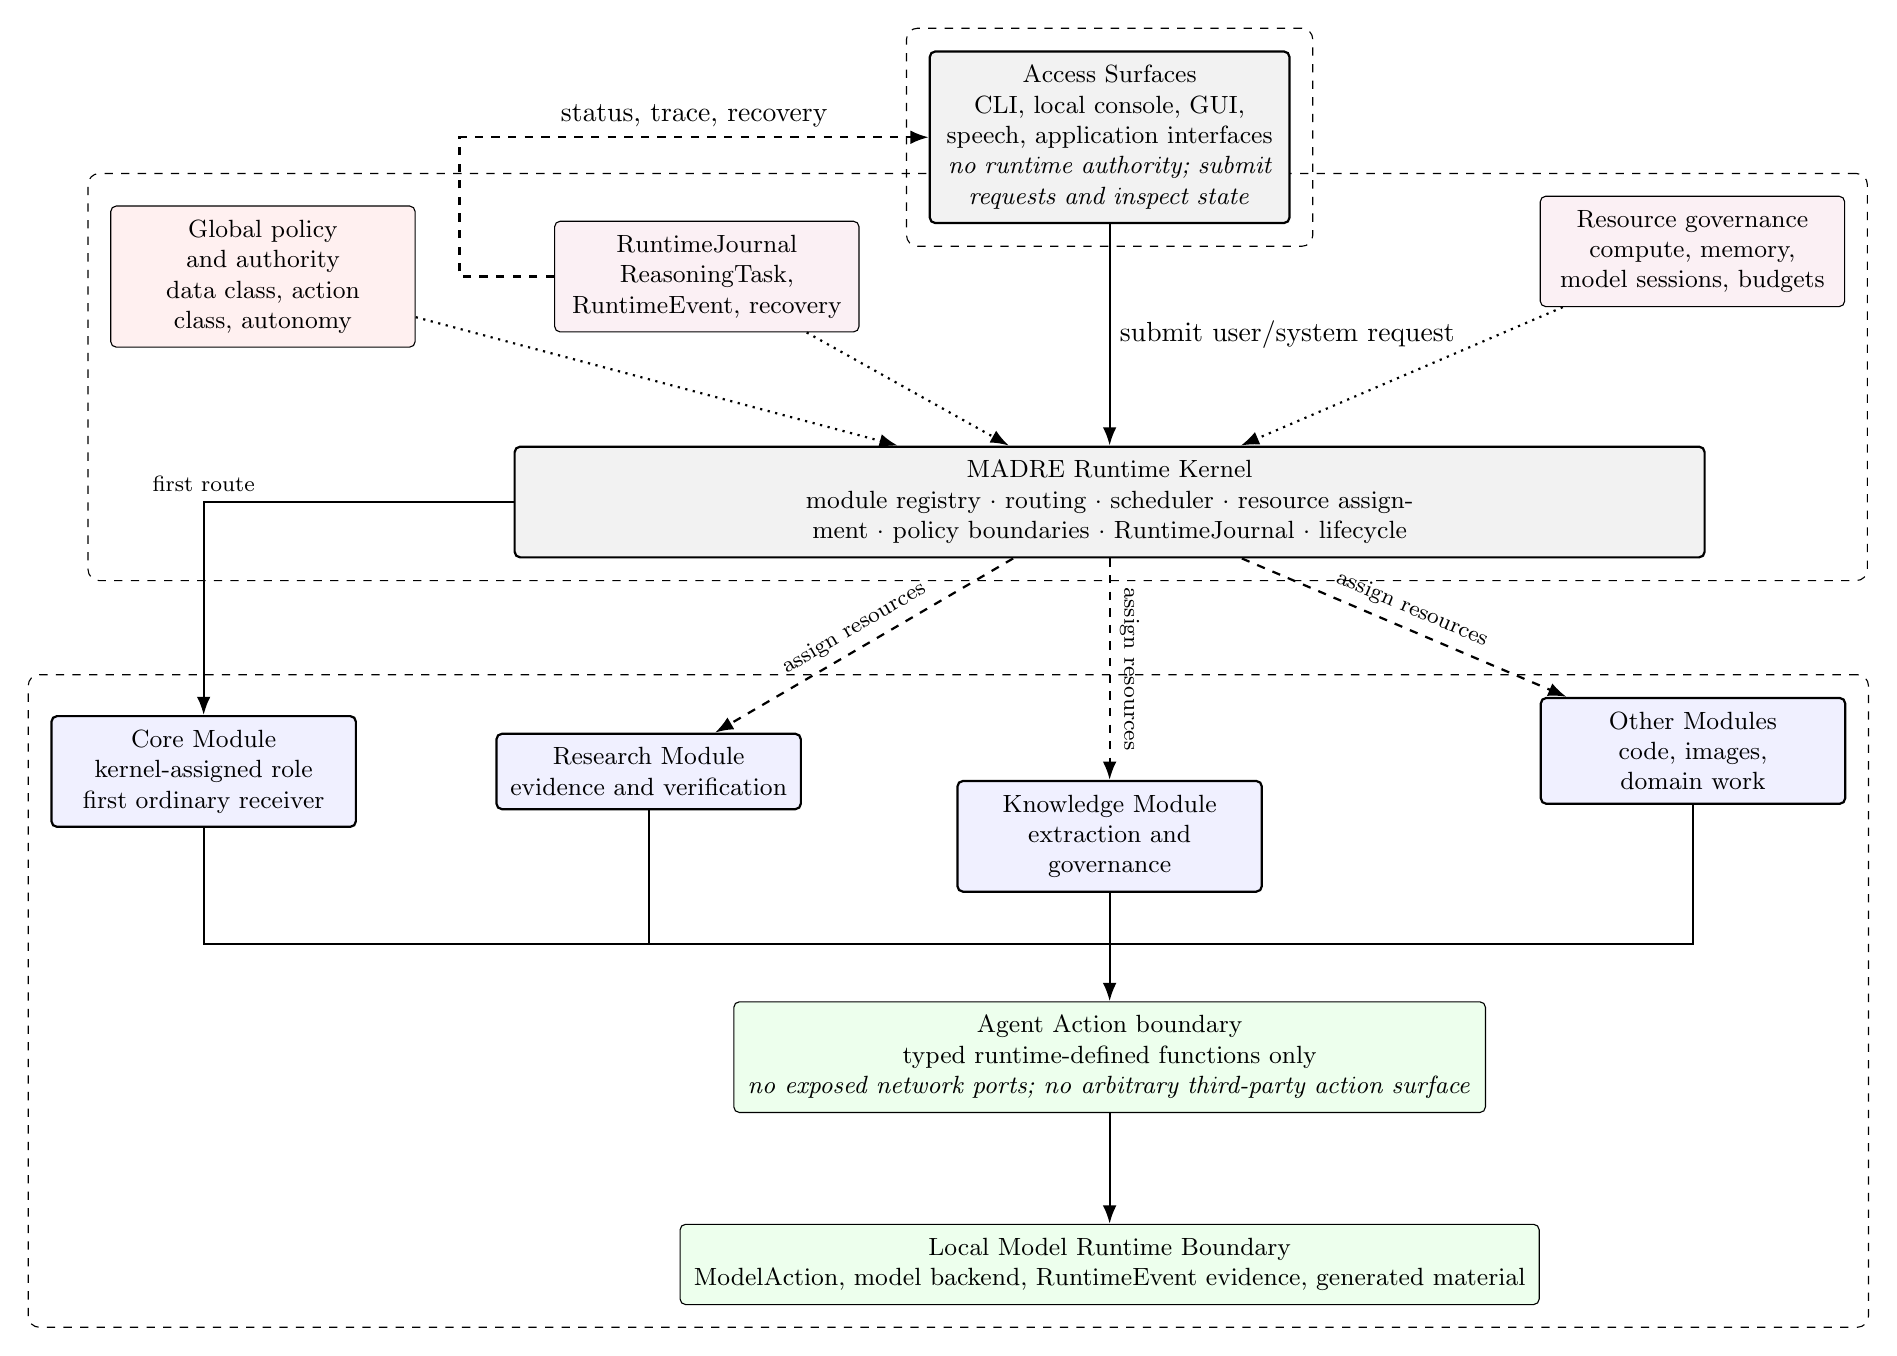
\begin{tikzpicture}[node distance=8em]

			% Access layer
			\node[madreKernel,text width=12em] (access)
			{Access Surfaces\\CLI, local console, GUI, speech, application interfaces\\
				\textit{no runtime authority; submit requests and inspect state}};

			% Kernel layer
			\node[madreKernel, below=of access, text width=42em, minimum height=3em] (kernel)
			{MADRE Runtime Kernel\\
				module registry $\cdot$ routing $\cdot$ scheduler $\cdot$ resource assignment $\cdot$ policy boundaries $\cdot$ RuntimeJournal $\cdot$ lifecycle};

			% Kernel owned services
			\node[madrePolicy, above left=5em of kernel, text width=10em] (policy)
			{Global policy and authority\\data class, action class, autonomy};
			\node[madreData, right=5em of policy, text width=10em] (state)
			{RuntimeJournal\\ReasoningTask, RuntimeEvent, recovery};
			\node[madreData, above right=5em and -6em of kernel, text width=10em] (resources)
			{Resource governance\\compute, memory, model sessions, budgets};

			% Module layer
			\node[madreModule, below left=of kernel, text width=10em] (core)
			{Core Module\\kernel-assigned role\\first ordinary receiver};
			\node[madreModule, right=5em of core, text width=10em] (research)
			{Research Module\\evidence and verification};
			\node[madreModule,  below right=5em and -6em of kernel, text width=10em] (domain){Other Modules\\code, images, domain work};
			\node[madreModule, below=of kernel, text width=10em] (knowledge){Knowledge Module\\extraction and governance};

			% Internal action layer
			\node[below=14em of kernel,line width=-.8em] (nodeactions){};
			\node[madreAction, below=16em of kernel, minimum width=8.5cm] (actions)
			{Agent Action boundary\\typed runtime-defined functions only\\
				\textit{no exposed network ports; no arbitrary third-party action surface}};

			% Model runtime layer
			\node[madreAction, below=4em of actions, minimum width=8.5cm] (models)
			{Local Model Runtime Boundary\\ModelAction, model backend, RuntimeEvent evidence, generated material};

			% Boundaries
			\begin{scope}[on background layer]
				\node[madreBoundary, fit=(access)] (b1) {};
				\node[madreBoundary, fit=(kernel)(policy)(state)(resources)] (b2) {};
				\node[madreBoundary, fit=(core)(research)(knowledge)(domain)(actions)(models)] (b3) {};
			\end{scope}

			% Flows
			\draw[madreFlow] (access) -- node[right]{submit user/system request} (kernel);
			\draw[madreFlow] (kernel) -| node[above]{ \footnotesize first route} (core);
			\draw[madreAsync] (kernel) -- node[above,sloped]{\footnotesize assign resources} (research);
			\draw[madreAsync] (kernel) -- node[above,sloped]{\footnotesize assign resources} (knowledge);
			\draw[madreAsync] (kernel) -- node[above,sloped]{\footnotesize assign resources} (domain);

			\draw[madreObserve] (policy) -- (kernel);
			\draw[madreObserve] (state) -- (kernel);
			\draw[madreObserve] (resources) -- (kernel);

			\draw[thick] (core) |- (nodeactions);
			\draw[thick] (research) |- (nodeactions);
			\draw[thick] (knowledge) |- (nodeactions);
			\draw[thick] (domain) |- (nodeactions);
			\draw[madreFlow] (nodeactions) -- (actions);
			\draw[madreFlow] (actions) -- (models);

			\draw[madreAsync] (state.west) -- ++(-1.2,0) |- node[near end, above]{status, trace, recovery} (access.west);

		\end{tikzpicture}%
	}
\caption{MADRE responsibility layers: kernel coordination, Core Module assignment, runtime journal, actions, and inference.}
	\label{fig:madre-responsibility-layers}
\end{figure}

Figure~\ref{fig:madre-responsibility-layers} defines the top-level responsibility model. Access surfaces are intentionally outside runtime authority: they submit requests and inspect state, but they do not own policy, knowledge, routing, scheduling, or action-authority decisions. The kernel is the only system-level coordinator. It registers modules, assigns the Core Module, routes requests, assigns resources, applies global policy boundaries, records through \texttt{RuntimeJournal}, and maintains durable lifecycle state.

The module layer is the reasoning layer. The Core Module is shown first because ordinary interaction is routed there by registration, not because it is outside the module system. Research, knowledge, code, media, or domain modules are peers selected when the registry, policies, and current reasoning plan indicate a better fit. Internal actions and inference appear below the module layer because they are invoked by authorized module behavior, not by access surfaces or generated material directly.

\begin{figure}[H]
	\centering
	\resizebox{0.92\linewidth}{!}{%
		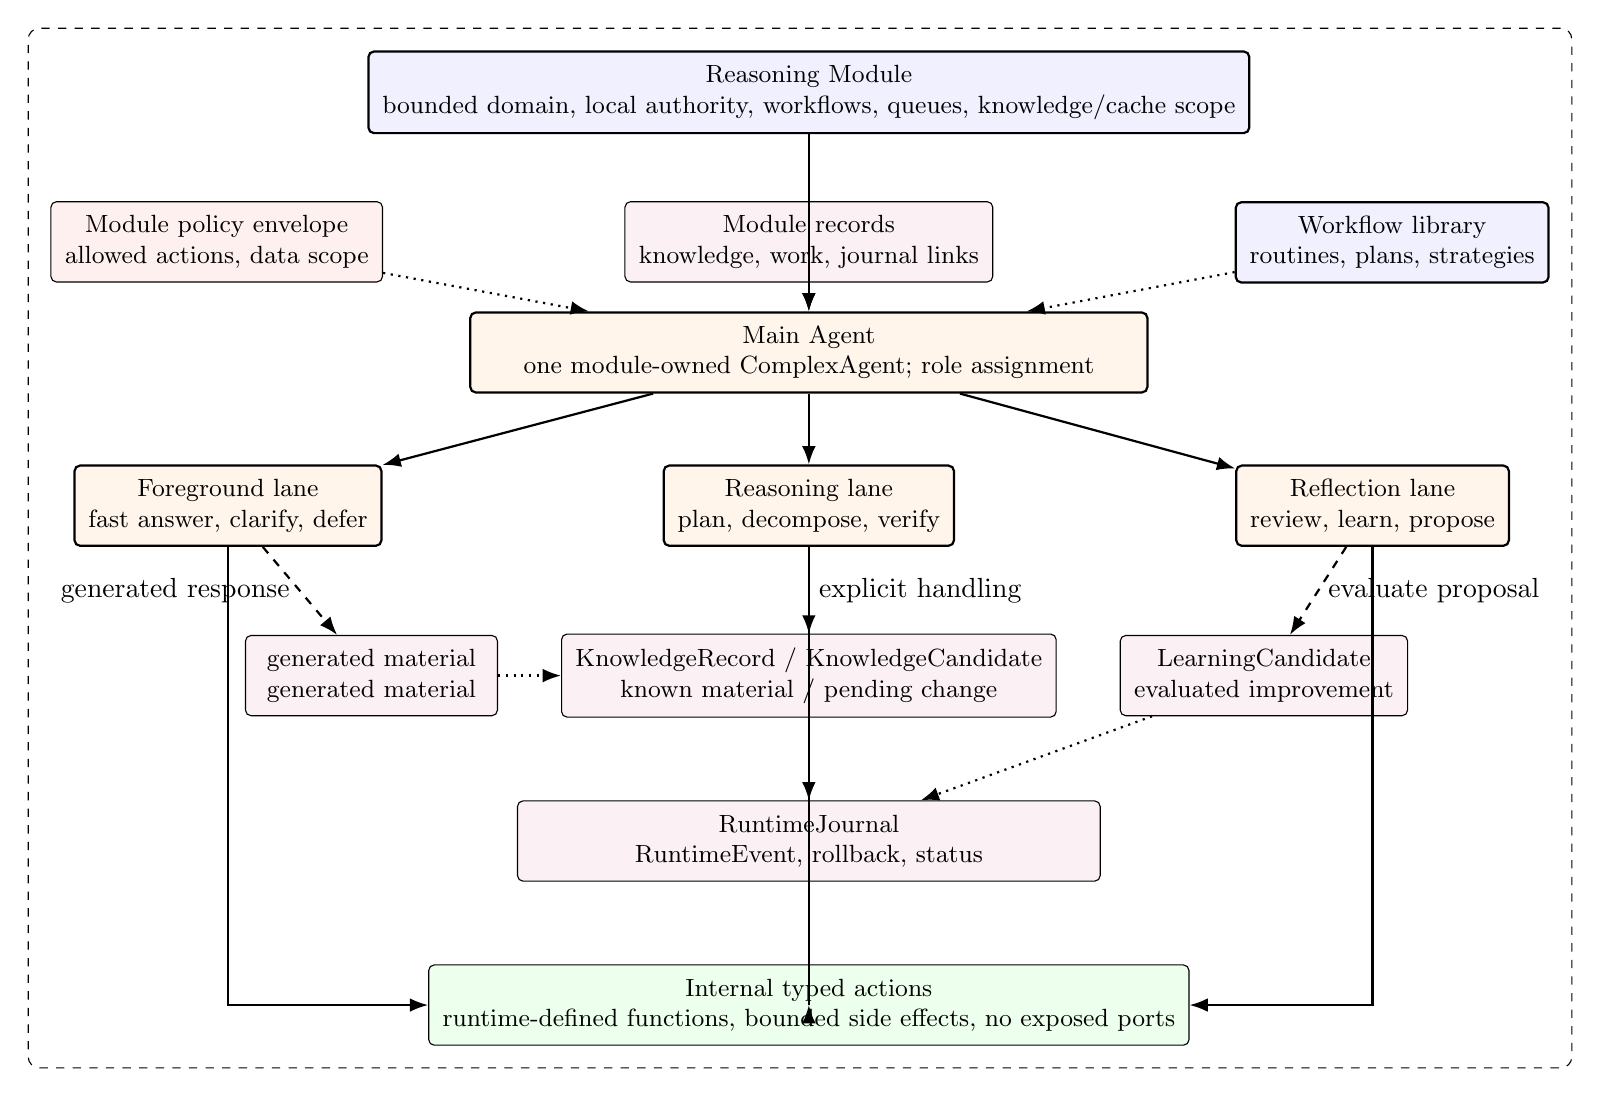
\begin{tikzpicture}[node distance=0.75cm and 0.95cm]

			% Module shell
			\node[madreModule, minimum width=8.8cm] (module)
			{Reasoning Module\\bounded domain, local authority, workflows, queues, knowledge/cache scope};

			% Module internals
			\node[madrePolicy, below left=0.85cm and -0.2cm of module, minimum width=3.2cm] (mpolicy)
			{Module policy envelope\\allowed actions, data scope};
			\node[madreData, below=0.85cm of module, minimum width=3.2cm] (mstate)
			{Module records\\knowledge, work, journal links};
			\node[madreModule, below right=0.85cm and -0.2cm of module, minimum width=3.2cm] (workflows)
			{Workflow library\\routines, plans, strategies};

			% Agent
			\node[madreAgent, below=2.25cm of module, minimum width=8.6cm, minimum height=0.95cm] (agent)
			{Main Agent\\one module-owned ComplexAgent; role assignment};

			% Triple lane
			\node[madreAgent, below left=0.9cm and 1.1cm of agent, minimum width=3.2cm] (fast)
			{Foreground lane\\fast answer, clarify, defer};
			\node[madreAgent, below=0.9cm of agent, minimum width=3.2cm] (deep)
			{Reasoning lane\\plan, decompose, verify};
			\node[madreAgent, below right=0.9cm and 1.1cm of agent, minimum width=3.2cm] (reflect)
			{Reflection lane\\review, learn, propose};

			% Runtime material and proposals
			\node[madreData, below=1.1cm of deep, minimum width=3.2cm] (knowledge)
			{KnowledgeRecord / KnowledgeCandidate\\known material / pending change};
			\node[madreData, left=0.8cm of knowledge, minimum width=3.2cm] (output)
			{generated material\\generated material};
			\node[madreData, right=0.8cm of knowledge, minimum width=3.2cm] (learning)
			{LearningCandidate\\evaluated improvement};
			\node[madreData, below=1.05cm of knowledge, minimum width=7.4cm] (journal)
			{RuntimeJournal\\RuntimeEvent, rollback, status};

			% Internal actions
			\node[madreAction, below=1.05cm of journal, minimum width=7.4cm] (iactions)
			{Internal typed actions\\runtime-defined functions, bounded side effects, no exposed ports};

			% Flows
			\draw[madreFlow] (module) -- (agent);
			\draw[madreObserve] (mpolicy) -- (agent);
			\draw[madreObserve] (mstate) -- (agent);
			\draw[madreObserve] (workflows) -- (agent);

			\draw[madreFlow] (agent) -- (fast);
			\draw[madreFlow] (agent) -- (deep);
			\draw[madreFlow] (agent) -- (reflect);

			\draw[madreAsync] (fast) -- node[left]{generated response} (output);
			\draw[madreAsync] (deep) -- node[right]{explicit handling} (knowledge);
			\draw[madreAsync] (reflect) -- node[right]{evaluate proposal} (learning);

			\draw[madreObserve] (output) -- (knowledge);
			\draw[madreObserve] (knowledge) -- (journal);
			\draw[madreObserve] (learning) -- (journal);

			\draw[madreFlow] (deep) |- (iactions);
			\draw[madreFlow] (reflect) |- (iactions);
			\draw[madreFlow] (fast) |- (iactions);

			% Boundary
			\begin{scope}[on background layer]
				\node[madreBoundary, fit=(module)(mpolicy)(mstate)(workflows)(agent)(fast)(deep)(reflect)(output)(knowledge)(learning)(journal)(iactions)] {};
			\end{scope}

		\end{tikzpicture}%
	}
	\caption{Reasoning module internal structure with its Main Agent using a ComplexAgent lane profile.}
	\label{fig:madre-complex-agent-module}
\end{figure}

Figure~\ref{fig:madre-complex-agent-module} expands the internal structure of a reasoning module. A module owns a bounded domain, local policy envelope, records, workflow library, knowledge boundary, and concrete \texttt{MADREAgent} objects. One module-owned \texttt{SystemAgent} holds the Main Agent role; additional \texttt{ComplexAgent} objects may serve other module work without that role.

The foreground lane, reasoning lane, and reflection lane may operate concurrently. The foreground lane protects user continuity. The reasoning lane protects evidence, decomposition, verification, and stronger work. The reflection lane protects adaptation by evaluating a proposed \texttt{LearningCandidate} rather than silently rewriting runtime behavior. These lanes do not increase agent authority. They remain constrained by module policy, kernel policy, assigned resources, trace requirements, and promotion boundaries.

\begin{figure}[H]
	\centering
	\resizebox{0.92\linewidth}{!}{%
		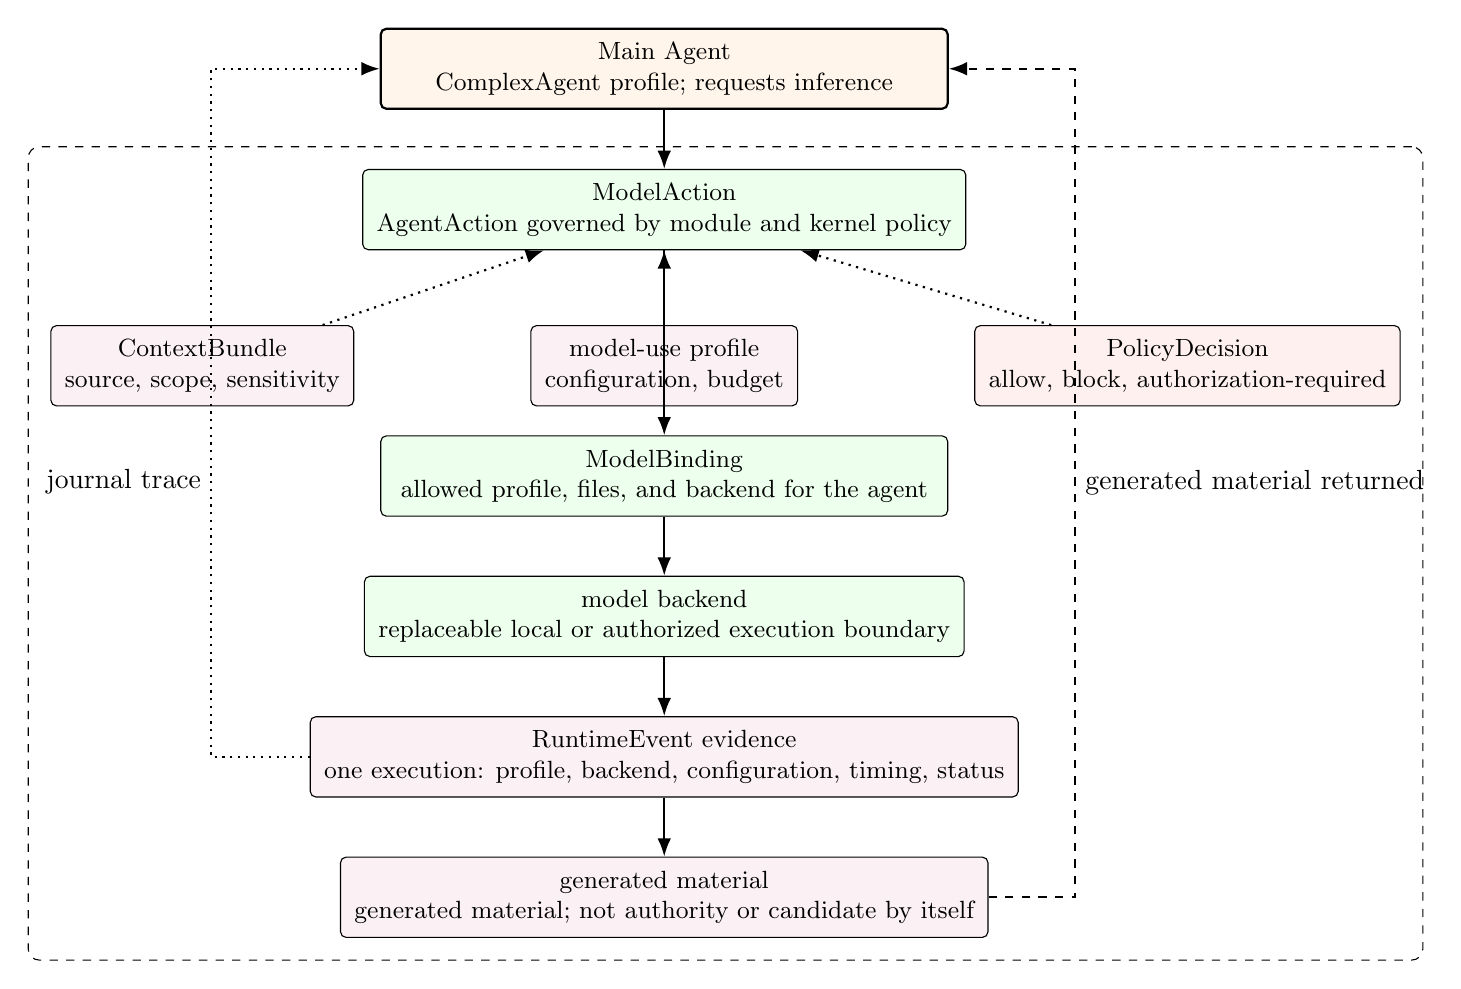
\begin{tikzpicture}[node distance=0.75cm and 0.9cm]

			% Caller
			\node[madreAgent, minimum width=7.2cm] (agent)
			{Main Agent\\ ComplexAgent profile; requests inference};

			\node[madreAction, below=of agent, minimum width=7.2cm] (action)
			{ModelAction\\AgentAction governed by module and kernel policy};

			% Governed inputs
			\node[madreData, below left=0.95cm and 0.1cm of action, minimum width=3.2cm] (ctx)
			{ContextBundle\\source, scope, sensitivity};
			\node[madreData, below=0.95cm of action, minimum width=3.2cm] (profile)
			{model-use profile\\configuration, budget};
			\node[madrePolicy, below right=0.95cm and 0.1cm of action, minimum width=3.2cm] (policy)
			{PolicyDecision\\allow, block, authorization-required};

			\node[madreAction, below=2.35cm of action, minimum width=7.2cm] (binding)
			{ModelBinding\\allowed profile, files, and backend for the agent};

			\node[madreAction, below=of binding, minimum width=7.2cm] (backend)
			{model backend\\replaceable local or authorized execution boundary};

			\node[madreData, below=of backend, minimum width=7.2cm] (record)
			{RuntimeEvent evidence\\one execution: profile, backend, configuration, timing, status};

			\node[madreData, below=of record, minimum width=7.2cm] (result)
			{generated material\\generated material; not authority or candidate by itself};

			% Flows
			\draw[madreFlow] (agent) -- (action);
			\draw[madreObserve] (ctx) -- (action);
			\draw[madreObserve] (profile) -- (action);
			\draw[madreObserve] (policy) -- (action);
			\draw[madreFlow] (action) -- (binding);
			\draw[madreFlow] (binding) -- (backend);
			\draw[madreFlow] (backend) -- (record);
			\draw[madreFlow] (record) -- (result);

			\draw[madreAsync] (result.east) -- ++(1.1,0) |- node[pos=0.25,right]{generated material returned} (agent.east);
			\draw[madreObserve] (record.west) -- ++(-1.25,0) |- node[pos=0.2,left]{journal trace} (agent.west);

			% Boundary
			\begin{scope}[on background layer]
				\node[madreBoundary, fit=(action)(ctx)(profile)(policy)(binding)(backend)(record)(result)] {};
			\end{scope}

		\end{tikzpicture}%
	}
	\caption{ModelAction inference path from governed execution through RuntimeEvent evidence to non-authoritative generated material.}
	\label{fig:madre-model-invocation-action}
\end{figure}

Figure~\ref{fig:madre-model-invocation-action} describes inference as the governed \texttt{ModelAction} path rather than as an external server call or chat-completion product boundary. A module-owned \texttt{MADREAgent}, including one serving as Main Agent role, can request generation, critique, classification, or verification only under its allowed \texttt{ModelBinding} and an applicable \texttt{PolicyDecision}.

The model-use profile captures execution configuration, and the replaceable model backend executes the permitted inference. Every execution creates an \texttt{RuntimeEvent} evidence; the generated material attached to that execution is generated material. The Local Model Runtime Boundary remains useful as product wording for this controlled local or authorized execution boundary, not as a competing runtime class. generated material is not truth, policy, memory, knowledge, behavior, routing, authority, or a candidate by itself. Explicit module handling can retain it as retained interaction material, save appropriately classified material as \texttt{KnowledgeRecord}, evaluate it toward a \texttt{LearningCandidate}, or discard it, with the transition recorded in \texttt{RuntimeJournal}.
\subsection{Data And Authority Rules}

\begin{itemize}
	\item User input enters as retained interaction material material when retained, not as policy, knowledge, truth, action authority, or model authority.
	\item Retrieved, extracted, or saved material becomes \texttt{KnowledgeRecord} only with provenance, scope, sensitivity, intended use, \texttt{truthLevel}, \texttt{truthAuthority}, correction, and lifecycle metadata; it is not factual truth by default.
	\item Context bundles are constructed, minimized, classified, scoped, and revocable before they reach an agent lane, internal action, or \texttt{ModelAction}.
	\item generated material is generated material from an \texttt{RuntimeEvent} evidence; it does not become an answer, policy decision, memory, knowledge, behavior, routing, authority, or candidate by itself.
	\item Internal action results enter as bounded observations. They become relied-on evidence only according to the action contract, verification path, and \texttt{RuntimeEvent} trace.
	\item External action surfaces, host commands, remote services, arbitrary filesystem mutation, credentials, and irreversible effects require stronger authority boundaries than ordinary internal actions.
	\item A \texttt{KnowledgeCandidate} represents only pending knowledge-boundary change; a \texttt{LearningCandidate} represents evaluated proposed module improvement and cannot directly rewrite active runtime behavior.
	\end{itemize}

\subsection{Trust Boundary Diagram}

The trust boundary diagram distinguishes the ordinary local governed domain from optional external or risky domains. The default execution path remains inside the local governed domain: access surfaces, kernel coordination, reasoning modules, internal typed actions, local model runtime, \texttt{RuntimeJournal}, and recovery.

The external boundary exists for exceptional external actions: remote services, provider-backed models, host-command execution, arbitrary filesystem mutation, network access, untrusted source acquisition, or third-party integrations. These are not ordinary internal actions. They require classification, minimization, explicit policy authorization, recorded trace, and a recovery or blocking expectation appropriate to their risk class.

\begin{center}
\resizebox{.95\linewidth}{!}{
\begin{tikzpicture}[
	zone/.style={draw, rounded corners=4pt, minimum width=4.1cm, minimum height=5.2cm, align=center},
	box/.style={draw, rounded corners=2pt, align=center, text width=3.2cm, minimum height=.85cm, inner sep=5pt},
	arrow/.style={-{Latex[length=2mm]}, thick}
]
	\node[zone, fill=secondaryColor!10] (local) at (0,0) {};
	\node[above] at (local.north) {\textbf{Local private domain}};
	\node[box] (private) at (0,1.4) {retained interaction material\\KnowledgeRecord};
	\node[box] (kernel) at (0,0) {MADRE kernel\\policy boundary};
	\node[box] (audit) at (0,-1.4) {RuntimeJournal\\recovery};

	\node[zone, fill=primaryColor!8] (boundary) at (5.4,0) {};
	\node[above] at (boundary.north) {\textbf{Governed external boundary}};
	\node[box] (classify) at (5.4,1.4) {Classify\\minimize\\redact};
	\node[box] (authorize) at (5.4,0) {Policy and\\authorization};
	\node[box] (contract) at (5.4,-1.4) {Typed runtime\\contract};

	\node[zone, fill=gray!8] (external) at (10.8,0) {};
	\node[above] at (external.north) {\textbf{External or risky domain}};
	\node[box] (remote) at (10.8,1.4) {Remote model\\or service};
	\node[box] (externalaction) at (10.8,0) {External action\\surface};
	\node[box] (source) at (10.8,-1.4) {Untrusted\\source material};

	\draw[arrow] (kernel) -- (classify);
	\draw[arrow] (classify) -- (authorize);
	\draw[arrow] (authorize) -- (contract);
	\draw[arrow] (contract) -- (remote);
	\draw[arrow] (contract) -- (externalaction);
	\draw[arrow] (source) -- (contract);
	\draw[arrow] (contract) -- (audit);
\end{tikzpicture}
}
\end{center}

\subsection{Access Surfaces}

\Madre exposes access surfaces without allowing those surfaces to define the kernel. The \texttt{madre} CLI submits local requests and exposes status or result evidence. A local read-first inspection console may expose sessions, queued work, context bundles, policy outcomes, model evidence, internal action evidence, \texttt{KnowledgeCandidate}, \texttt{LearningCandidate}, \texttt{RuntimeJournal} traces, recovery, and runtime state. These surfaces operate under the same policy and authority model as every other runtime interaction.

The inspection console is not a privileged mutation path. Its transport is intentionally not fixed at architecture level. If a later implementation uses HTTP, sockets, embedded UI, or another mechanism, that choice must be justified by deployment and security decisions and must preserve local-first, read-first, policy-governed behavior.

Graphical, speech, product-specific, or integration surfaces remain access surfaces over the runtime rather than privileged paths around it.

\madreChapter{Design Decision Traceability}

Design decisions D-001 through D-011 provide traceability from product
requirements to architecture obligations and validation evidence. They identify
accepted product architecture decisions for governed delayed reasoning, durable
work, context, inference, policy, recovery, bounded internal actions, local access,
knowledge-boundary control, and evaluated learning promotion.

\MADRETABLE3:{\textbf{Decision} & \textbf{Product-level effect} & \textbf{Architecture boundary}}{
	D-001 & Defines source-backed delayed-answer behavior as a core expression of governed runtime value. & Conversation remains connected to durable work and evidence. \N
	D-002 & Establishes behavior-first architectural validation as part of the product's engineering discipline. & Observable behavior anchors architecture claims. \N
	D-003 & Requires \texttt{ReasoningTask} lifecycle and projected inspection state. & \texttt{RuntimeJournal} and append-only \texttt{RuntimeEvent} preserve local traceability. \N
	D-004 & Requires conservative foreground triage. & Unsupported answers become clarification, policy block, or delayed work. \N
	D-005 & Requires governed context acceptance and rejection. & Context is sourced, classified, minimized, scoped, provenanced, and revocable. \N
	D-006 & Requires \texttt{ModelAction}, model backend, \texttt{RuntimeEvent} evidence, and non-authoritative generated material. & Models remain runtime functions, not authorities or candidate creators by generation alone. \N
	D-007 & Requires explicit \texttt{PolicyDecision} before action execution. & Action execution follows policy rather than model instruction. \N
	D-008 & Requires recovery as a recorded semantic transition. & Correction, rollback, invalidation, supersession, deletion, and detachment have distinguishable \texttt{RuntimeEvent} meaning. \N
	D-009 & Defines bounded internal actions as the low-risk executable reference. & Action execution is policy-gated, traceable, and recoverability-aware. \N
	D-010 & Defines CLI request/status interaction and local read-first console inspection as canonical local access surfaces. & Access surfaces expose the kernel without becoming runtime authority. \N
	D-011 & Distinguishes pending \texttt{KnowledgeCandidate} boundary changes from evaluated \texttt{LearningCandidate} module improvements. & Known-material storage is not learning; proposed evolution remains inspectable until promoted by authority. }

\madreChapter{Architecture Viewpoints}

\section{Viewpoint Catalogue}

\MADRETABLE3:{\textbf{Viewpoint} & \textbf{Primary concern} & \textbf{MADRE content} }{%
	System context & Runtime boundary and environment & User, local device, filesystem, operating system, local models, optional external integrations, internal actions, and untrusted sources. \N
	Logical & Responsibility separation & Kernel, Core Module, module-owned agents, scheduler, context/knowledge, Local Model Runtime Boundary, Agent Action boundary, \texttt{PolicyDecision}, \texttt{RuntimeJournal}, learning, and recovery. \N
	Runtime/process & Work lifecycle & User turn, triage, \texttt{ReasoningTask}, context bundle, scheduling, \texttt{RuntimeEvent} evidence, result delivery, \texttt{RuntimeEvent}, and recovery. \N
	Data/knowledge & Data ownership and provenance & retained interaction material, \texttt{KnowledgeRecord}, \texttt{KnowledgeCandidate}, \texttt{LearningCandidate}, truth metadata, retention, correction, and deletion. \N
	Security/trust & Boundary enforcement & Local domain, governed external boundary, external/risky domain, prompt injection, remote transfer, credential exposure, and action side effects. \N
	Deployment & Local operation & Ordinary device profile, local storage, model availability, backup, migration, diagnostics, and optional remote configuration. \N
	Extension & Developer evolution & \texttt{ModelBinding}, model-use profile, model backend, action contracts, workflows, projections, context policies, and interface surfaces. \N
	UX & User-visible control & Conversation, clarification, queue state, progress, authorization, failure, completion, correction, and rollback.}

\section{Viewpoint Design Focus}


\MADRETABLE3:{
	\textbf{Viewpoint} & \textbf{Architecture focus} & \textbf{Authority boundary} }{
	System context & Local user, local device, CLI, local read-first console, local sources, and optional remote integrations. & Local authority remains explicit across every access surface. \N
	Logical & Kernel coordination over routing, delayed work, context, bounded action use, \texttt{PolicyDecision}, \texttt{RuntimeJournal}, and recovery. & Runtime authority is not delegated to interfaces, models, actions, or generated material. \N
	Runtime/process & Governed lifecycle from local request to inspection and recovery. & \texttt{ReasoningTask} transitions remain recorded, inspectable, and recoverable. \N
	Data/knowledge & Governed context and explicit knowledge/learning types. & Source material, retained interaction material, \texttt{KnowledgeRecord}, \texttt{KnowledgeCandidate}, and \texttt{LearningCandidate} remain distinguishable. \N
	Security/trust & Source-as-data, model-as-function, policy before action, and bounded internal action authority. & Action execution follows declared policy outcomes. \N
	Observability/recovery & Local status, \texttt{RuntimeJournal}, verification, policy, knowledge/learning transition, and recovery evidence. & Read-first inspection must not become a privileged mutation path. \N
	Extension & Inference backends, actions, workflows, and learning systems inherit the defined boundaries. & Extension preserves kernel authority and product traceability. }
